%\documentclass[10pt]{beamer}
%\usefonttheme[onlylarge]{structurebold}

\documentclass[handout]{beamer}
\usefonttheme[onlylarge]{structurebold}
  \usepackage{pgfpages}
\mode<handout>
\pgfpagesuselayout{4 on 1}[letterpaper,border shrink=5mm]

\hypersetup{
  bookmarks = false,
  colorlinks,
  citecolor = red,
  linkcolor=blue,
  pdfpagemode=none,
  pdfstartview={Fit},
  pdftitle={},
  pdfauthor={Michael E. Waugh},
  pdfkeywords={} }
  \setbeamertemplate{navigation symbols}{}

\mode<presentation> {
  \usetheme{boxes}
  % or ...

  \setbeamercovered{transparent}
  % or whatever (possibly just delete it)
}

\setbeamertemplate{itemize subitem}[circle]
\setbeamerfont{frametitle}{size= \large}
\setbeamerfont{ framesubtitle }{size = \footnotesize}
\setbeamertemplate{frametitle}
{
\medskip
\smallskip
{\textsf{\underline{\insertframetitle\phantom{))))))))}}}}}


\usepackage[english]{babel}
\usepackage{wasysym}

\addfootbox{}{\hspace{5cm}\tiny {Macroeconomic Data | Economics of Global Business, Revised: \today}}%

\title[NYU Stern] % (optional, use only with long paper titles)
{\huge Macroeconomic Data}

\author[Michael Waugh] % (optional, use only with lots of authors)
{\bf{\Large}}%

\date[] % (optional)

\subject{Talks}

\begin{document}

\begin{frame}
  \titlepage
\end{frame}

%%%%%%%%%%%%%%%%%%%%%%%%%%%%%%%%%%%%%%%%%%%%%%%%%%%%%%%%%%%%%%%%%%%%%%%%%%%%%%%%%%%%%%%%%%%%%%%%
%%%%%%%%%%%%%%%%%%%%%%%%%%%%%%%%%%%%%%%%%%%%%%%%%%%%%%%%%%%%%%%%%%%%%%%%%%%%%%%%%%%%%%%%%%%%%%%%

\begin{frame}[t]
\frametitle{The Plan}
\begin{itemize}
\item Overview of macroeconomic data\ldots
\begin{itemize}
\medskip
\item GDP: What it is, How it's measured.
\medskip
\item Real vs. Nominal: Separating prices from quantities.
\medskip
\item Measuring labor market performance.
\medskip
\item FRED: How to get data.
\end{itemize}
\end{itemize}
\bigskip
\end{frame}

%%%%%%%%%%%%%%%%%%%%%%%%%%%%%%%%%%%%%%%%%%%%%%%%%%%%%%%%%%%%%%%%%%%%%%%%%%%%%%%%%%%%%%%%%%%%%%%%%
%%%%%%%%%%%%%%%%%%%%%%%%%%%%%%%%%%%%%%%%%%%%%%%%%%%%%%%%%%%%%%%%%%%%%%%%%%%%%%%%%%%%%%%%%%%%%%%%%
%
%\begin{frame}[t]
%\frametitle{Measurement: The Idea}
%\begin{itemize}
%\item Why worry about measurement?
%\begin{itemize}
%\medskip
%\item Need a common vocabulary
%\medskip
%\item Small changes in definition can make big differences
%\medskip
%\item Accurate forecasting requires consistent measurements
%\end{itemize}
%\end{itemize}
%\bigskip
%\end{frame}

%%%%%%%%%%%%%%%%%%%%%%%%%%%%%%%%%%%%%%%%%%%%%%%%%%%%%%%%%%%%%%%%%%%%%%%%%%%%%%%%%%%%%%%%%%%%%%%%
%%%%%%%%%%%%%%%%%%%%%%%%%%%%%%%%%%%%%%%%%%%%%%%%%%%%%%%%%%%%%%%%%%%%%%%%%%%%%%%%%%%%%%%%%%%%%%%%
\begin{frame}[t]
\frametitle{GDP}
\begin{itemize}
\item GDP = Gross Domestic Product
\bigskip
\item GDP = the market value of final goods and services newly produced within a nation during a fixed period of time.
\begin{itemize}
\medskip
\item \textbf{Market value }(it allows to add up different products, but misses home production; black economy; non-traded government services)
\medskip
\item \textbf{New goods} (i.e., not second-hand exchanges)
\medskip
\item \textbf{Within a nation}: domestic location (not citizenship)
\medskip
\item A measure of \textbf{final} goods and services (why? See next slide)
\medskip
\item \textbf{Gross} of depreciation, i.e., it does not embody capital consumption due to wear and tear (Example: reduction in value of a car used by a taxi company)
\end{itemize}
\end{itemize}
\bigskip
\end{frame}

%%%%%%%%%%%%%%%%%%%%%%%%%%%%%%%%%%%%%%%%%%%%%%%%%%%%%%%%%%%%%%%%%%%%%%%%%%%%%%%%%%%%%%%%%%%%%%%%
%%%%%%%%%%%%%%%%%%%%%%%%%%%%%%%%%%%%%%%%%%%%%%%%%%%%%%%%%%%%%%%%%%%%%%%%%%%%%%%%%%%%%%%%%%%%%%%%

\begin{frame}[t]
\frametitle{Three Ways to Compute GDP}
How to compute GDP:
\begin{itemize}
\medskip
\item GDP = Value added: Sales minus material input costs (intermediate inputs).
\bigskip
\item GDP = Income: Payments to labor and capital (profits, rental income).
\bigskip
\item GDP = Expenditure: Purchases of final goods and services, including exports minus imports
\end{itemize}
\bigskip
\end{frame}

%%%%%%%%%%%%%%%%%%%%%%%%%%%%%%%%%%%%%%%%%%%%%%%%%%%%%%%%%%%%%%%%%%%%%%%%%%%%%%%%%%%%%%%%%%%%%%%%
%%%%%%%%%%%%%%%%%%%%%%%%%%%%%%%%%%%%%%%%%%%%%%%%%%%%%%%%%%%%%%%%%%%%%%%%%%%%%%%%%%%%%%%%%%%%%%%%

\begin{frame}[t]
\frametitle{GDP as Value Added}
\begin{itemize}
\item Value added $=$ sales $-$ material input costs
\bigskip
\item Example
\begin{itemize}
\medskip
\item Farmer produces wheat, sells it for 100
\medskip
\item Miller buys wheat, produces flour, sells it for 175
\medskip
\item Baker buys flour, makes bread, sells it for 300
\end{itemize}
\bigskip
\item What is value added for each producer?
\bigskip
\item What is GDP?
\end{itemize}
\bigskip
\end{frame}

%%%%%%%%%%%%%%%%%%%%%%%%%%%%%%%%%%%%%%%%%%%%%%%%%%%%%%%%%%%%%%%%%%%%%%%%%%%%%%%%%%%%%%%%%%%%%%%%
%%%%%%%%%%%%%%%%%%%%%%%%%%%%%%%%%%%%%%%%%%%%%%%%%%%%%%%%%%%%%%%%%%%%%%%%%%%%%%%%%%%%%%%%%%%%%%%%

\begin{frame}[t]
\frametitle{Intermediate vs Final Goods}
\begin{itemize}
\item Why not sum over all goods?
\begin{itemize}
\medskip
\item TO AVOID DOUBLE COUNTING!
\end{itemize}
\bigskip
\item Another example:
\begin{itemize}
\medskip
\item Goodrich Corporation manufactures and sells components and systems for aircraft. Say that it produces just one system per year for Boeing, worth \$10M.
\medskip
\item Boeing buys the system for its 787 aircraft; total value of the airplane is \$80M.
\medskip
\item The landing system produced by Goodrich is included in the \$80M! The value of the final good (the airplane) includes the value of the intermediate parts (engines, frame,  navigation system, etc.)
\end{itemize}
\end{itemize}
\bigskip
\end{frame}

%%%%%%%%%%%%%%%%%%%%%%%%%%%%%%%%%%%%%%%%%%%%%%%%%%%%%%%%%%%%%%%%%%%%%%%%%%%%%%%%%%%%%%%%%%%%%%%%
%%%%%%%%%%%%%%%%%%%%%%%%%%%%%%%%%%%%%%%%%%%%%%%%%%%%%%%%%%%%%%%%%%%%%%%%%%%%%%%%%%%%%%%%%%%%%%%%

\begin{frame}[t]
\frametitle{GDP as Income}
\begin{itemize}
\item GDP = payments to labor and capital
\bigskip
\item In income but not in GDP
\begin{itemize}
\medskip
\item Capital gains
\medskip
\item Interest on government debt
\medskip
\item Net foreign income
\end{itemize}
\bigskip
\item In GDP but not in income
\begin{itemize}
\medskip
\item Depreciation
\end{itemize}
\bigskip
\item Bottom line GDP $\thickapprox$ income
\end{itemize}
\end{frame}

%%%%%%%%%%%%%%%%%%%%%%%%%%%%%%%%%%%%%%%%%%%%%%%%%%%%%%%%%%%%%%%%%%%%%%%%%%%%%%%%%%%%%%%%%%%%%%%%
%%%%%%%%%%%%%%%%%%%%%%%%%%%%%%%%%%%%%%%%%%%%%%%%%%%%%%%%%%%%%%%%%%%%%%%%%%%%%%%%%%%%%%%%%%%%%%%%

\begin{frame}[t]
\frametitle{GDP as Final Sales}
\begin{itemize}
\item GDP = purchases of final goods and services, including exports minus imports
\bigskip
\item Final goods/service purchases broken down in the following way\ldots\\
\medskip
GDP = C + I + G + NX.
\begin{itemize}
\medskip
\item C = final sales new goods to households, ``consumption''
\medskip
\item I = final sales of new capital goods to firms, ``investment''
\medskip
\item G = purchases of new goods and services by government
\medskip
\item NX = net exports, exports - imports
\end{itemize}
\end{itemize}
\end{frame}

%%%%%%%%%%%%%%%%%%%%%%%%%%%%%%%%%%%%%%%%%%%%%%%%%%%%%%%%%%%%%%%%%%%%%%%%%%%%%%%%%%%%%%%%%%%%%%%%
%%%%%%%%%%%%%%%%%%%%%%%%%%%%%%%%%%%%%%%%%%%%%%%%%%%%%%%%%%%%%%%%%%%%%%%%%%%%%%%%%%%%%%%%%%%%%%%%

\begin{frame}[t]
\frametitle{More on Consumption, Investment, etc.}
\begin{itemize}
\item C = final sales new goods to households, ``consumption''
\begin{itemize}
\medskip
\item Includes, things like durable (i.e. long lasting) goods, nondurables, services.
\end{itemize}
\medskip
\item I = final sales of new capital goods to firms, ``investment''
\begin{itemize}
\medskip
\item That is a physical asset used by firms in future production.
\medskip
\item Includes: Firms spending on plant and equipment, residential spending by consumers and landlords on housing, change firms inventories
\end{itemize}
\medskip
\item G = purchases of new goods and services by government
\begin{itemize}
\medskip
\item Does NOT include transfer payments (i.e. food stamps/unemploymen insurance).
\end{itemize}
\end{itemize}
\end{frame}

%%%%%%%%%%%%%%%%%%%%%%%%%%%%%%%%%%%%%%%%%%%%%%%%%%%%%%%%%%%%%%%%%%%%%%%%%%%%%%%%%%%%%%%%%%%%%%%%
%%%%%%%%%%%%%%%%%%%%%%%%%%%%%%%%%%%%%%%%%%%%%%%%%%%%%%%%%%%%%%%%%%%%%%%%%%%%%%%%%%%%%%%%%%%%%%%%

\begin{frame}[t]
\frametitle{Problems in Measuring GDP}
\begin{itemize}
\item How to measure government services?
\begin{itemize}
\smallskip
\item Valued at cost, i.e. use the second approach (income side) to measure GDP.
\end{itemize}
\bigskip
\item Ignores household production
\bigskip
\item Ignores intangible investment
\bigskip
\item Ignores ``underground'' economy
\bigskip
\item Environment/Pollution
\bigskip
\item Separate point --- the formula $Y = C+I+G+NX$ says nothing about causality.
\end{itemize}
\end{frame}

%%%%%%%%%%%%%%%%%%%%%%%%%%%%%%%%%%%%%%%%%%%%%%%%%%%%%%%%%%%%%%%%%%%%%%%%%%%%%%%%%%%%%%%%%%%%%%%%
%%%%%%%%%%%%%%%%%%%%%%%%%%%%%%%%%%%%%%%%%%%%%%%%%%%%%%%%%%%%%%%%%%%%%%%%%%%%%%%%%%%%%%%%%%%%%%%%

\begin{frame}[t]
\frametitle{GDP Identities}
\bigskip
\bigskip
\begin{itemize}
\item Now try the extended example.
\end{itemize}
\end{frame}

%%%%%%%%%%%%%%%%%%%%%%%%%%%%%%%%%%%%%%%%%%%%%%%%%%%%%%%%%%%%%%%%%%%%%%%%%%%%%%%%%%%%%%%%%%%%%%%%
%%%%%%%%%%%%%%%%%%%%%%%%%%%%%%%%%%%%%%%%%%%%%%%%%%%%%%%%%%%%%%%%%%%%%%%%%%%%%%%%%%%%%%%%%%%%%%%%

\begin{frame}[t]
\frametitle{Prices and Quantities}
\begin{itemize}
\item We would like to measure changes in \ldots
\begin{itemize}
\medskip
\item quantities over time
\medskip
\item quantities across countries
\medskip
\item price changes over time
\end{itemize}
\bigskip
\item Problem:
\begin{itemize}
\medskip
\item many goods in the economy
\medskip
\item relative prices change across time
\medskip
\item relative prices are different across locations
\end{itemize}
\end{itemize}
\end{frame}

%%%%%%%%%%%%%%%%%%%%%%%%%%%%%%%%%%%%%%%%%%%%%%%%%%%%%%%%%%%%%%%%%%%%%%%%%%%%%%%%%%%%%%%%%%%%%%%%
%%%%%%%%%%%%%%%%%%%%%%%%%%%%%%%%%%%%%%%%%%%%%%%%%%%%%%%%%%%%%%%%%%%%%%%%%%%%%%%%%%%%%%%%%%%%%%%%

\begin{frame}[t]
\frametitle{Language Prices and Quantities}
\begin{itemize}
\item Terminology
\begin{itemize}
\medskip
\item GDP at current prices: ``nominal'' (value = price $\times$ quantity)
\medskip
\item GDP at base-year prices: ``real'' (quantity)
\medskip
\item GDP at PPP adjusted prices: ``real'' (quantity)
\end{itemize}
\bigskip
\item Ok, how to we go from ``nominal'' to ``real''?
\end{itemize}
\end{frame}

%%%%%%%%%%%%%%%%%%%%%%%%%%%%%%%%%%%%%%%%%%%%%%%%%%%%%%%%%%%%%%%%%%%%%%%%%%%%%%%%%%%%%%%%%%%%%%%%
%%%%%%%%%%%%%%%%%%%%%%%%%%%%%%%%%%%%%%%%%%%%%%%%%%%%%%%%%%%%%%%%%%%%%%%%%%%%%%%%%%%%%%%%%%%%%%%%

\begin{frame}[t]
\frametitle{With only one good: no problem!}
\begin{itemize}

\item GDP {\it equals} price {\it times} quantity:

\begin{equation*}
Y_t=p_t\times q_t
\end{equation*}
\medskip

\item Growth rate in GDP {\it equals} growth rate in price {\it times} growth rate in quantity %

\begin{equation*}
\frac{Y_t}{Y_{t-1}}=\frac{p_t
q_t}{p_{t-1}q_{t-1}}=\frac{p_t}{p_{t-1}}\times\frac{q_t}{q_{t-1}}
\end{equation*}
\end{itemize}
\end{frame}

%%%%%%%%%%%%%%%%%%%%%%%%%%%%%%%%%%%%%%%%%%%%%%%%%%%%%%%%%%%%%%%%%%%%%%%%%%%%%%%%%%%%%%%%%%%%%%%%
%%%%%%%%%%%%%%%%%%%%%%%%%%%%%%%%%%%%%%%%%%%%%%%%%%%%%%%%%%%%%%%%%%%%%%%%%%%%%%%%%%%%%%%%%%%%%%%%

\begin{frame}[t]
\frametitle{With multiple goods?}
\begin{table}[t]
\setlength {\tabcolsep}{3.75mm}
\vspace{0.01cm}
\renewcommand{\arraystretch}{1.5}
\begin{center}
\begin{tabular}{l|c c |c c }
\hline
\hline
& \multicolumn{2}{c}{Fish}& \multicolumn{2}{c}{Chips}\\
\hline
Date & Price & Quantity & Price & Quantity \ \\
\hline
2016 & 0.50  & 10 & 0.25  & 10\\
2017  & 0.75 & 12 & 0.50 & 8\\
\hline
\hline
\end{tabular}
\end{center}
\end{table}
\only<2>{
\bigskip
\smallskip
\begin{itemize}
\item The problem is that relative prices change!
\medskip
\item How to we go from ``nominal'' to ``real''? Two ways to do this \ldots
\begin{itemize}
\medskip
\item GDP Deflator
\medskip
\item Consumer Price Index (Mankiw 2-2).
\end{itemize}
\end{itemize}}
\end{frame}


%%%%%%%%%%%%%%%%%%%%%%%%%%%%%%%%%%%%%%%%%%%%%%%%%%%%%%%%%%%%%%%%%%%%%%%%%%%%%%%%%%%%%%%%%%%%%%%%
%%%%%%%%%%%%%%%%%%%%%%%%%%%%%%%%%%%%%%%%%%%%%%%%%%%%%%%%%%%%%%%%%%%%%%%%%%%%%%%%%%%%%%%%%%%%%%%%

\begin{frame}[t]
\frametitle{Approach \#1: GDP Deflator Approach}
\begin{itemize}
\item Basic Idea
\begin{itemize}
\medskip
\item Pick a base year
\medskip
\item Evaluate current year quantities at base year prices
\begin{eqnarray*}
\mbox{2017 \ Real \ GDP \ in 2016 \ dollars} = p_{f,2016}q_{f,2017} + p_{c,2016}q_{c,2017}
\end{eqnarray*}
\end{itemize}
\bigskip
\item To compute inflation?
\begin{itemize}
\medskip
\item Compute the Price Deflator  = $\frac{\mbox{Nominal  \ GDP}}{\mbox{Real  \ GDP}}$.
\bigskip
\item Inflation is the \textbf{growth rate} of the price deflator.
\end{itemize}
\end{itemize}
\end{frame}

%%%%%%%%%%%%%%%%%%%%%%%%%%%%%%%%%%%%%%%%%%%%%%%%%%%%%%%%%%%%%%%%%%%%%%%%%%%%%%%%%%%%%%%%%%%%%%%%
%%%%%%%%%%%%%%%%%%%%%%%%%%%%%%%%%%%%%%%%%%%%%%%%%%%%%%%%%%%%%%%%%%%%%%%%%%%%%%%%%%%%%%%%%%%%%%%%


\begin{frame}[t]
\frametitle{GDP Deflator Approach}
\begin{table}[t]
\setlength {\tabcolsep}{3.75mm}
\vspace{0.01cm}
\renewcommand{\arraystretch}{1.25}
\begin{center}
\begin{tabular}{l|c c |c c }
\hline
\hline
& \multicolumn{2}{c}{Fish}& \multicolumn{2}{c}{Chips}\\
\hline
Date & Price & Quantity & Price & Quantity \ \\
\hline
2016 & 0.50  & 10 & 0.25  & 10\\
2017  & 0.75 & 12 & 0.50 & 8\\
\hline
\hline
\end{tabular}
\end{center}
\end{table}

\medskip
\begin{itemize}
\item 2016 GDP
\begin{eqnarray*}
\mbox{Nominal \ GDP} = 0.50\times10 + 0.25\times10 = 7.5\\
\mbox{Real \ GDP} = 0.50\times10 + 0.25\times10 = 7.5
\end{eqnarray*}
\item 2017 GDP
\begin{eqnarray*}
\mbox{Nominal \ GDP} = 0.75\times12 + 0.50\times8 = 13.0\\
\mbox{Real \ GDP} = \begin{alertenv}{\textbf{0.50}}\end{alertenv}\times12 + \begin{alertenv}{\textbf{0.25}}\end{alertenv}\times8 = \phantom{1}8.0
\end{eqnarray*}
\end{itemize}
\end{frame}

%%%%%%%%%%%%%%%%%%%%%%%%%%%%%%%%%%%%%%%%%%%%%%%%%%%%%%%%%%%%%%%%%%%%%%%%%%%%%%%%%%%%%%%%%%%%%%%%
%%%%%%%%%%%%%%%%%%%%%%%%%%%%%%%%%%%%%%%%%%%%%%%%%%%%%%%%%%%%%%%%%%%%%%%%%%%%%%%%%%%%%%%%%%%%%%%%

\begin{frame}[t]
\frametitle{GDP Deflator Approach}
\begin{table}[t]
\setlength {\tabcolsep}{3.75mm}
\vspace{0.01cm}
\renewcommand{\arraystretch}{1.25}
\begin{center}
\begin{tabular}{l|c c |c c }
\hline
\hline
& \multicolumn{2}{c}{Fish}& \multicolumn{2}{c}{Chips}\\
\hline
Date & Price & Quantity & Price & Quantity \ \\
\hline
2016 & 0.50  & 10 & 0.25  & 10\\
2017  & 0.75 & 12 & 0.50 & 8\\
\hline
\hline
\end{tabular}
\end{center}
\end{table}
\medskip
\begin{itemize}
\item \begin{alertenv}{Real GDP Growth in percent}\end{alertenv}
\begin{eqnarray*}
100\times\left(\ln (\mbox{2017 \ Real \ GDP}) - \ln (\mbox{2016 \ Real \ GDP}) \right) = \phantom{6.45} \\
\\
100\times\left(\ln (8.0) - \ln (7.5) \right) = 6.45
\end{eqnarray*}
\end{itemize}
\end{frame}

%%%%%%%%%%%%%%%%%%%%%%%%%%%%%%%%%%%%%%%%%%%%%%%%%%%%%%%%%%%%%%%%%%%%%%%%%%%%%%%%%%%%%%%%%%%%%%%%
%%%%%%%%%%%%%%%%%%%%%%%%%%%%%%%%%%%%%%%%%%%%%%%%%%%%%%%%%%%%%%%%%%%%%%%%%%%%%%%%%%%%%%%%%%%%%%%%


\begin{frame}[t]
\frametitle{GDP Deflator Approach}
\begin{table}[t]
\setlength {\tabcolsep}{3.75mm}
\vspace{0.01cm}
\renewcommand{\arraystretch}{1.25}
\begin{center}
\begin{tabular}{l|c c |c c }
\hline
\hline
& \multicolumn{2}{c}{Fish}& \multicolumn{2}{c}{Chips}\\
\hline
Date & Price & Quantity & Price & Quantity \ \\
\hline
2016 & 0.50  & 10 & 0.25  & 10\\
2017  & 0.75 & 12 & 0.50 & 8\\
\hline
\hline
\end{tabular}
\end{center}
\end{table}
\medskip
\begin{itemize}
\item Price Deflator
\begin{eqnarray*}
2016 \mbox{\ P.D.} = \frac{\mbox{2016 \ Nominal \ GDP}}{\mbox{2016 \ Real \ GDP}}= 1\phantom{.625}\\
\\
2017 \mbox{\ P.D.}= \frac{\mbox{2017 \ Nominal \ GDP}}{\mbox{2017 \ Real \ GDP}}= 1.625\\
\end{eqnarray*}
\end{itemize}
\end{frame}

%%%%%%%%%%%%%%%%%%%%%%%%%%%%%%%%%%%%%%%%%%%%%%%%%%%%%%%%%%%%%%%%%%%%%%%%%%%%%%%%%%%%%%%%%%%%%%%%
%%%%%%%%%%%%%%%%%%%%%%%%%%%%%%%%%%%%%%%%%%%%%%%%%%%%%%%%%%%%%%%%%%%%%%%%%%%%%%%%%%%%%%%%%%%%%%%%

\begin{frame}[t]
\frametitle{GDP Deflator Approach}
\begin{table}[t]
\setlength {\tabcolsep}{3.75mm}
\vspace{0.01cm}
\renewcommand{\arraystretch}{1.25}
\begin{center}
\begin{tabular}{l|c c |c c }
\hline
\hline
& \multicolumn{2}{c}{Fish}& \multicolumn{2}{c}{Chips}\\
\hline
Date & Price & Quantity & Price & Quantity \ \\
\hline
2016 & 0.50  & 10 & 0.25  & 10\\
2017  & 0.75 & 12 & 0.50 & 8\\
\hline
\hline
\end{tabular}
\end{center}
\end{table}
\medskip
\begin{itemize}
\item \begin{alertenv}{Inflation in percent}\end{alertenv}
\begin{eqnarray*}
100\times\left(\ln (\mbox{2017 \ P.D.}) - \ln (\mbox{2016 \ P.D.}) \right) = \phantom{6.45} \\
\\
100\times\left(\ln (1.625) - \ln (1) \right) = 48.6
\end{eqnarray*}
\end{itemize}
\end{frame}

%%%%%%%%%%%%%%%%%%%%%%%%%%%%%%%%%%%%%%%%%%%%%%%%%%%%%%%%%%%%%%%%%%%%%%%%%%%%%%%%%%%%%%%%%%%%%%%%
%%%%%%%%%%%%%%%%%%%%%%%%%%%%%%%%%%%%%%%%%%%%%%%%%%%%%%%%%%%%%%%%%%%%%%%%%%%%%%%%%%%%%%%%%%%%%%%%

\begin{frame}[t]
\frametitle{Approach \#2: CPI-Price Index Approach}
\begin{itemize}
\item Basic Idea
\begin{itemize}
\medskip
\item Pick a base year
\medskip
\item Construct a price index and evaluate current year prices at base year quantities:
\begin{eqnarray*}
\mbox{2017 \ Price \ Index \ in 2016 \ dollars} = p_{f,2017}q_{f,2016} + p_{c,2017}q_{c,2016}
\end{eqnarray*}
\end{itemize}
\bigskip
\bigskip
\item See Mankiw 2-2. Work through this at home.
\end{itemize}
\end{frame}

%%%%%%%%%%%%%%%%%%%%%%%%%%%%%%%%%%%%%%%%%%%%%%%%%%%%%%%%%%%%%%%%%%%%%%%%%%%%%%%%%%%%%%%%%%%%%%%%
%%%%%%%%%%%%%%%%%%%%%%%%%%%%%%%%%%%%%%%%%%%%%%%%%%%%%%%%%%%%%%%%%%%%%%%%%%%%%%%%%%%%%%%%%%%%%%%%


\begin{frame}[t]
\frametitle{CPI-Price Index Approach}
\begin{table}[t]
\setlength {\tabcolsep}{3.75mm}
\vspace{0.01cm}
\renewcommand{\arraystretch}{1.25}
\begin{center}
\begin{tabular}{l|c c |c c }
\hline
\hline
& \multicolumn{2}{c}{Fish}& \multicolumn{2}{c}{Chips}\\
\hline
Date & Price & Quantity & Price & Quantity \ \\
\hline
2016 & 0.50  & 10 & 0.25  & 10\\
2017  & 0.75 & 12 & 0.50 & 8\\
\hline
\hline
\end{tabular}
\end{center}
\end{table}
\medskip
\begin{eqnarray*}
\mbox{2016 \ Price \ Index} = 0.50\times10 + 0.25\times10 = 7.5
\end{eqnarray*}
\begin{eqnarray*}
\mbox{2017 \ Price \ Index} = 0.75\times\begin{alertenv}{\textbf{10}}\end{alertenv} + 0.50\times\begin{alertenv}{\textbf{10}}\end{alertenv} = 12.5
\end{eqnarray*}
\end{frame}

%%%%%%%%%%%%%%%%%%%%%%%%%%%%%%%%%%%%%%%%%%%%%%%%%%%%%%%%%%%%%%%%%%%%%%%%%%%%%%%%%%%%%%%%%%%%%%%%
%%%%%%%%%%%%%%%%%%%%%%%%%%%%%%%%%%%%%%%%%%%%%%%%%%%%%%%%%%%%%%%%%%%%%%%%%%%%%%%%%%%%%%%%%%%%%%%%


\begin{frame}[t]
\frametitle{CPI-Price Index Approach}
\begin{table}[t]
\setlength {\tabcolsep}{3.75mm}
\vspace{0.01cm}
\renewcommand{\arraystretch}{1.25}
\begin{center}
\begin{tabular}{l|c c |c c }
\hline
\hline
& \multicolumn{2}{c}{Fish}& \multicolumn{2}{c}{Chips}\\
\hline
Date & Price & Quantity & Price & Quantity \ \\
\hline
2016 & 0.50  & 10 & 0.25  & 10\\
2017  & 0.75 & 12 & 0.50 & 8\\
\hline
\hline
\end{tabular}
\end{center}
\end{table}
\medskip
\begin{itemize}
\item \begin{alertenv}{Inflation in percent}\end{alertenv}
\begin{eqnarray*}
100\times\left(\ln (\mbox{2017 \ Price \ Index}) - \ln (\mbox{2016 \ Price \ Index}) \right) = \phantom{6.45} \\
\\
100\times\left(\ln (12.5) - \ln (7.5) \right) = 51.1
\end{eqnarray*}
\end{itemize}
\end{frame}

%%%%%%%%%%%%%%%%%%%%%%%%%%%%%%%%%%%%%%%%%%%%%%%%%%%%%%%%%%%%%%%%%%%%%%%%%%%%%%%%%%%%%%%%%%%%%%%%
%%%%%%%%%%%%%%%%%%%%%%%%%%%%%%%%%%%%%%%%%%%%%%%%%%%%%%%%%%%%%%%%%%%%%%%%%%%%%%%%%%%%%%%%%%%%%%%%


\begin{frame}[t]
\frametitle{Composition of the US CPI�s ``basket''}
\begin{center}
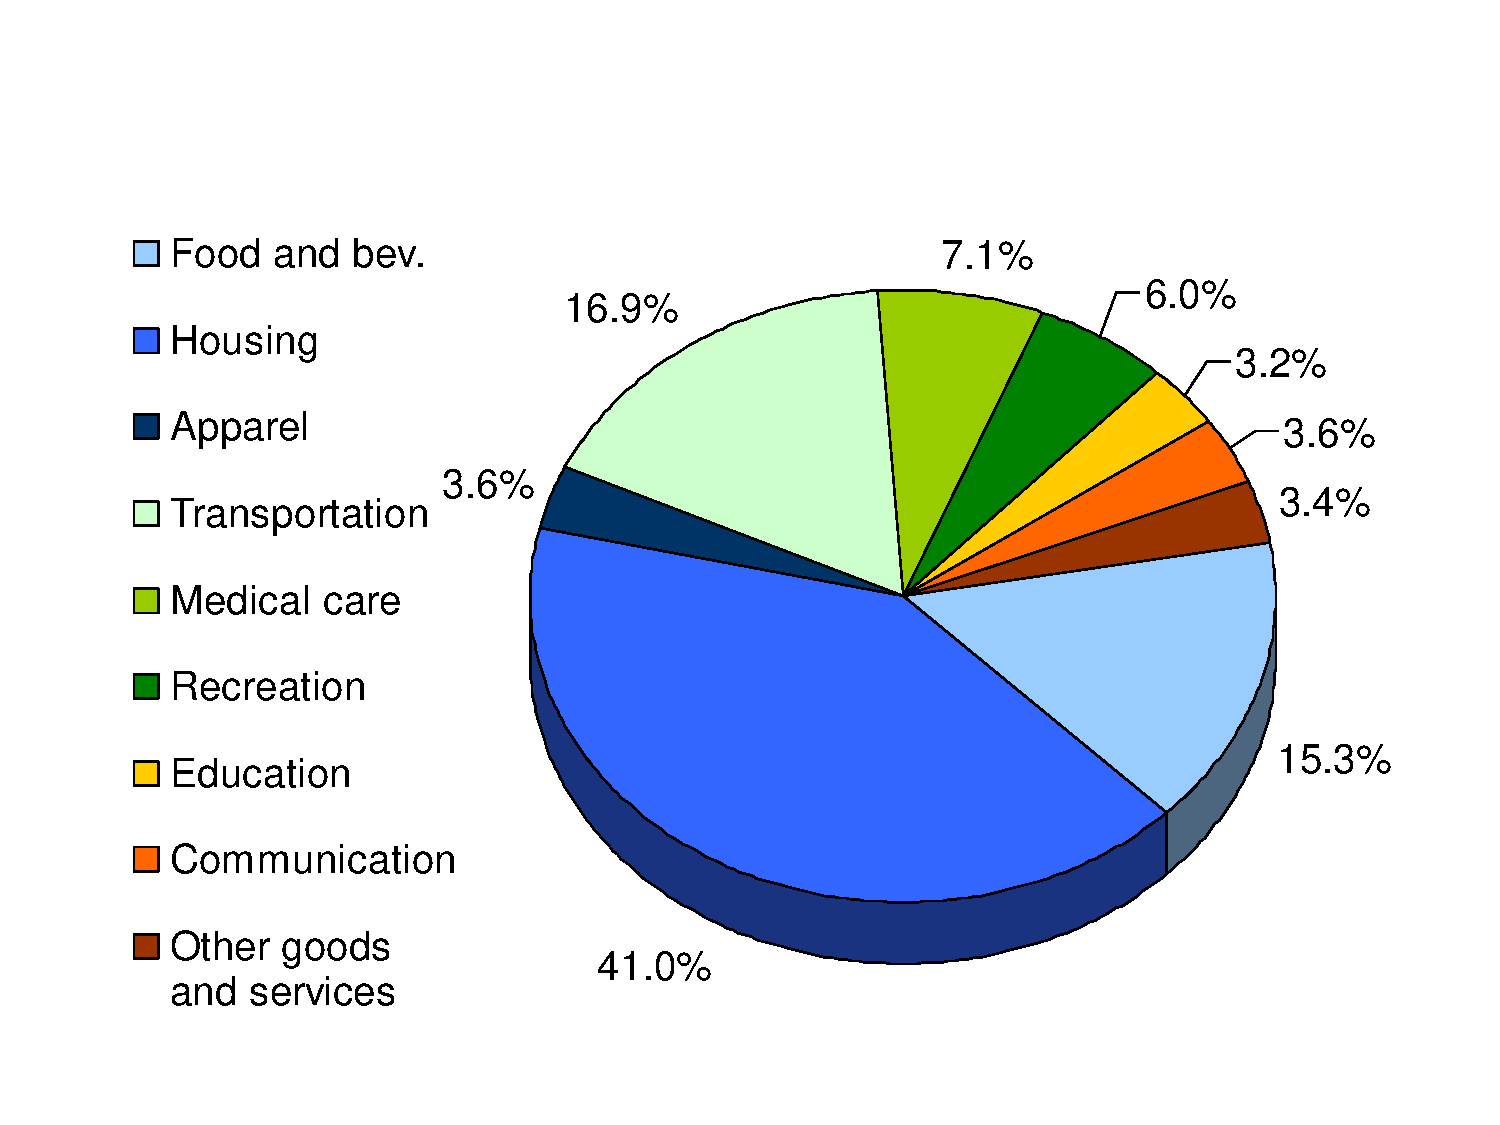
\includegraphics[height=3.1in,width=4.25in]{../figures/cpi_basket}
\end{center}
\end{frame}

%%%%%%%%%%%%%%%%%%%%%%%%%%%%%%%%%%%%%%%%%%%%%%%%%%%%%%%%%%%%%%%%%%%%%%%%%%%%%%%%%%%%%%%%%%%%%%%%
%%%%%%%%%%%%%%%%%%%%%%%%%%%%%%%%%%%%%%%%%%%%%%%%%%%%%%%%%%%%%%%%%%%%%%%%%%%%%%%%%%%%%%%%%%%%%%%%

\begin{frame}[t]
\frametitle{GDP Price Deflator vs CPI}
Three key conceptual differences\ldots
\begin{itemize}
\item GDP price deflator measures changes in prices for entire economy.\\
    \medskip
     CPI only measures prices of goods and services bought by consumers.
\bigskip
\item GDP price deflator only measures changes in prices for domestic production. International effects are netted out.\\
    \medskip
    CPI includes both domestically and imported goods.
\bigskip
\item More subtle. They are different types of price indexes. \\
    \medskip
GDP price deflator, the basket of goods can change. It will not completely reflect the costs of higher prices. \\
    \medskip
CPI fixes the basket, but prices change. It will not reflect substitution effects as relative prices change.
\end{itemize}
\end{frame}

%%%%%%%%%%%%%%%%%%%%%%%%%%%%%%%%%%%%%%%%%%%%%%%%%%%%%%%%%%%%%%%%%%%%%%%%%%%%%%%%%%%%%%%%%%%%%%%%
%%%%%%%%%%%%%%%%%%%%%%%%%%%%%%%%%%%%%%%%%%%%%%%%%%%%%%%%%%%%%%%%%%%%%%%%%%%%%%%%%%%%%%%%%%%%%%%%

\begin{frame}[t]
\frametitle{GDP Price Deflator vs CPI}
\begin{center}
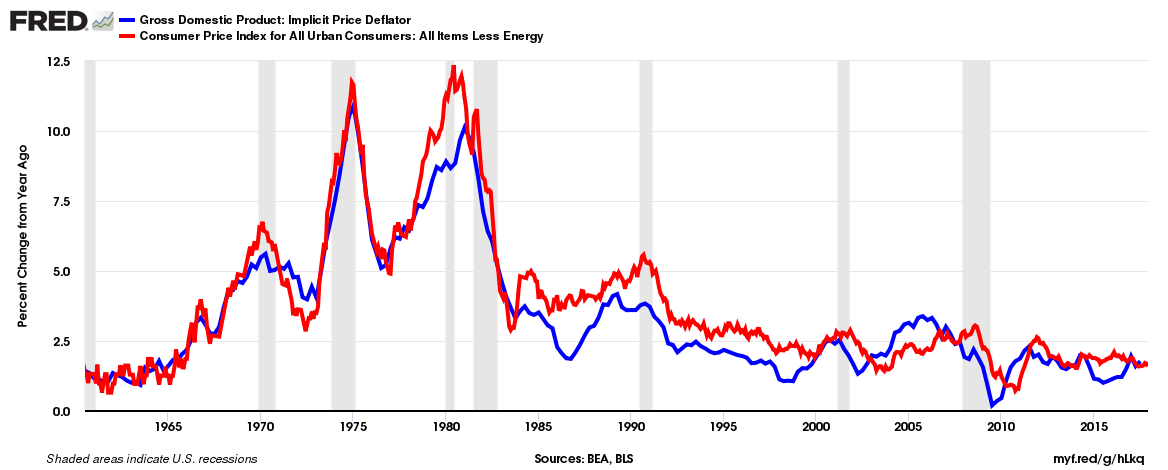
\includegraphics[height=3in,width=4.5in]{../figures/gdp_vs_cpi}
\end{center}
\end{frame}

%%%%%%%%%%%%%%%%%%%%%%%%%%%%%%%%%%%%%%%%%%%%%%%%%%%%%%%%%%%%%%%%%%%%%%%%%%%%%%%%%%%%%%%%%%%%%%%%
%%%%%%%%%%%%%%%%%%%%%%%%%%%%%%%%%%%%%%%%%%%%%%%%%%%%%%%%%%%%%%%%%%%%%%%%%%%%%%%%%%%%%%%%%%%%%%%%

\begin{frame}[t]
\frametitle{Cross-Country Comparisons}
\begin{itemize}
\item Same problem as before: Prices differ across countries, but we want to compare quantities
\bigskip
\item Similar solutions
\begin{itemize}
\medskip
\item Most common: Evaluate quantities at a common set of prices
\medskip
\item PPP = ``Purchasing Power Adjustment''
\end{itemize}
\end{itemize}
\end{frame}


%%%%%%%%%%%%%%%%%%%%%%%%%%%%%%%%%%%%%%%%%%%%%%%%%%%%%%%%%%%%%%%%%%%%%%%%%%%%%%%%%%%%%%%%%%%%%%%%
%%%%%%%%%%%%%%%%%%%%%%%%%%%%%%%%%%%%%%%%%%%%%%%%%%%%%%%%%%%%%%%%%%%%%%%%%%%%%%%%%%%%%%%%%%%%%%%%

\begin{frame}[t]
\frametitle{Measuring the Performance of the Labor Market\ldots}
Categories of the population
\begin{itemize}
\medskip
\item Employed: working at a paid job
\bigskip
\item Unemployed:not employed but looking for a job
\bigskip
\item Labor force: the amount of labor available for producing goods and services; employed plus unemployed
\bigskip
\item Not in the labor force: not employed, not looking for work
\end{itemize}
\end{frame}

%%%%%%%%%%%%%%%%%%%%%%%%%%%%%%%%%%%%%%%%%%%%%%%%%%%%%%%%%%%%%%%%%%%%%%%%%%%%%%%%%%%%%%%%%%%%%%%%
%%%%%%%%%%%%%%%%%%%%%%%%%%%%%%%%%%%%%%%%%%%%%%%%%%%%%%%%%%%%%%%%%%%%%%%%%%%%%%%%%%%%%%%%%%%%%%%%
\begin{frame}[t]
\frametitle{The Unemployment Rate and Labor Force Participation\ldots}
Two important labor force concepts
\begin{itemize}
\medskip
\item Unemployment rate: percentage of the labor force that is unemployed
\begin{align*}
= 100 \times \frac{\mbox{Unemployed}}{\mbox{Labor force}}
\end{align*}
\item Labor force participation rate: the fraction of the adult population that ``participates'' in the labor force, i.e. is working or looking for work
\begin{align*}
= 100 \times \frac{\mbox{Labor force}}{\mbox{Labor force} + \mbox{Not in Labor Force}}
\end{align*}
\end{itemize}
\end{frame}
%%%%%%%%%%%%%%%%%%%%%%%%%%%%%%%%%%%%%%%%%%%%%%%%%%%%%%%%%%%%%%%%%%%%%%%%%%%%%%%%%%%%%%%%%%%%%%%%
%%%%%%%%%%%%%%%%%%%%%%%%%%%%%%%%%%%%%%%%%%%%%%%%%%%%%%%%%%%%%%%%%%%%%%%%%%%%%%%%%%%%%%%%%%%%%%%%

\begin{frame}[t]
\frametitle{US Unemployment Rate}
\begin{center}
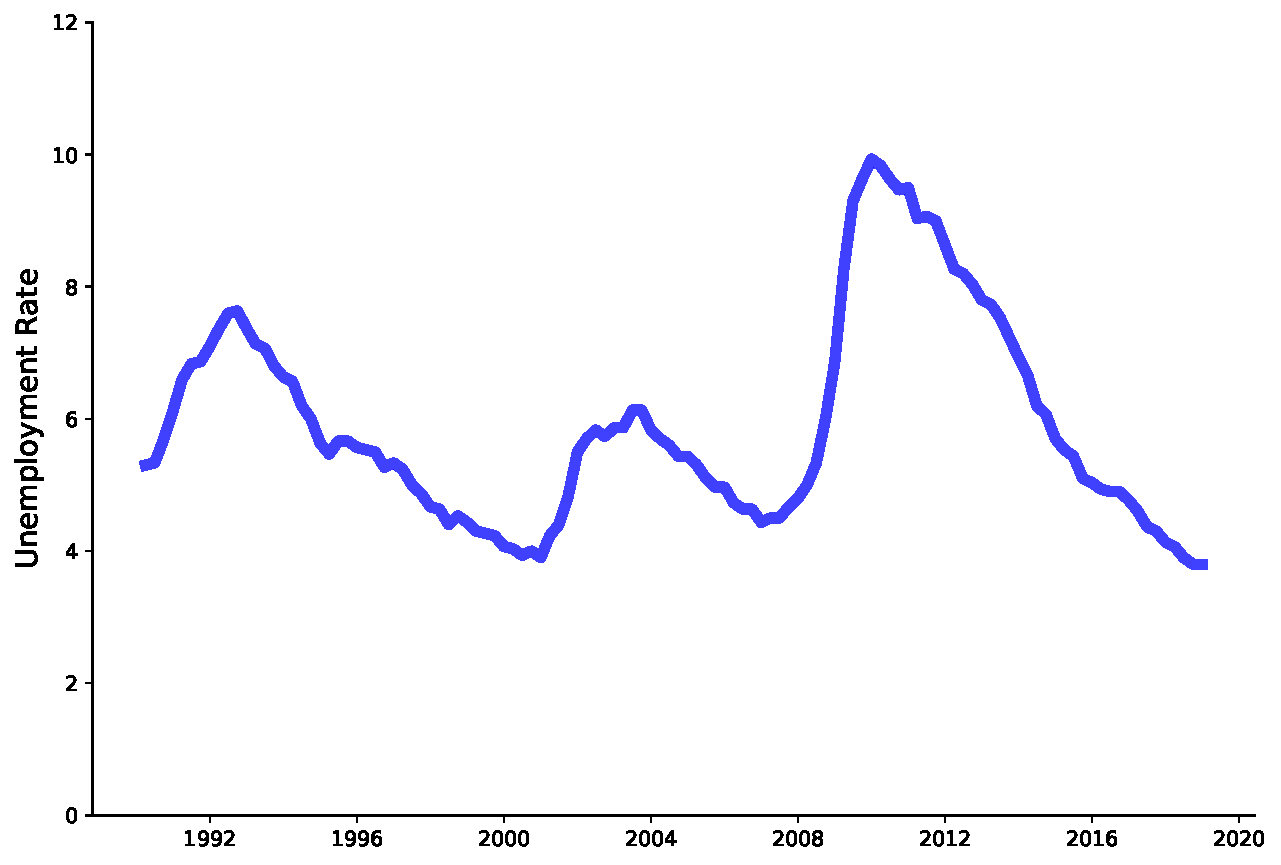
\includegraphics[scale = 0.5]{../figures/unemployment_rate}
\end{center}
\end{frame}

%%%%%%%%%%%%%%%%%%%%%%%%%%%%%%%%%%%%%%%%%%%%%%%%%%%%%%%%%%%%%%%%%%%%%%%%%%%%%%%%%%%%%%%%%%%%%%%%
%%%%%%%%%%%%%%%%%%%%%%%%%%%%%%%%%%%%%%%%%%%%%%%%%%%%%%%%%%%%%%%%%%%%%%%%%%%%%%%%%%%%%%%%%%%%%%%%


\begin{frame}[t]
\frametitle{US Labor Force Participation}
\begin{center}
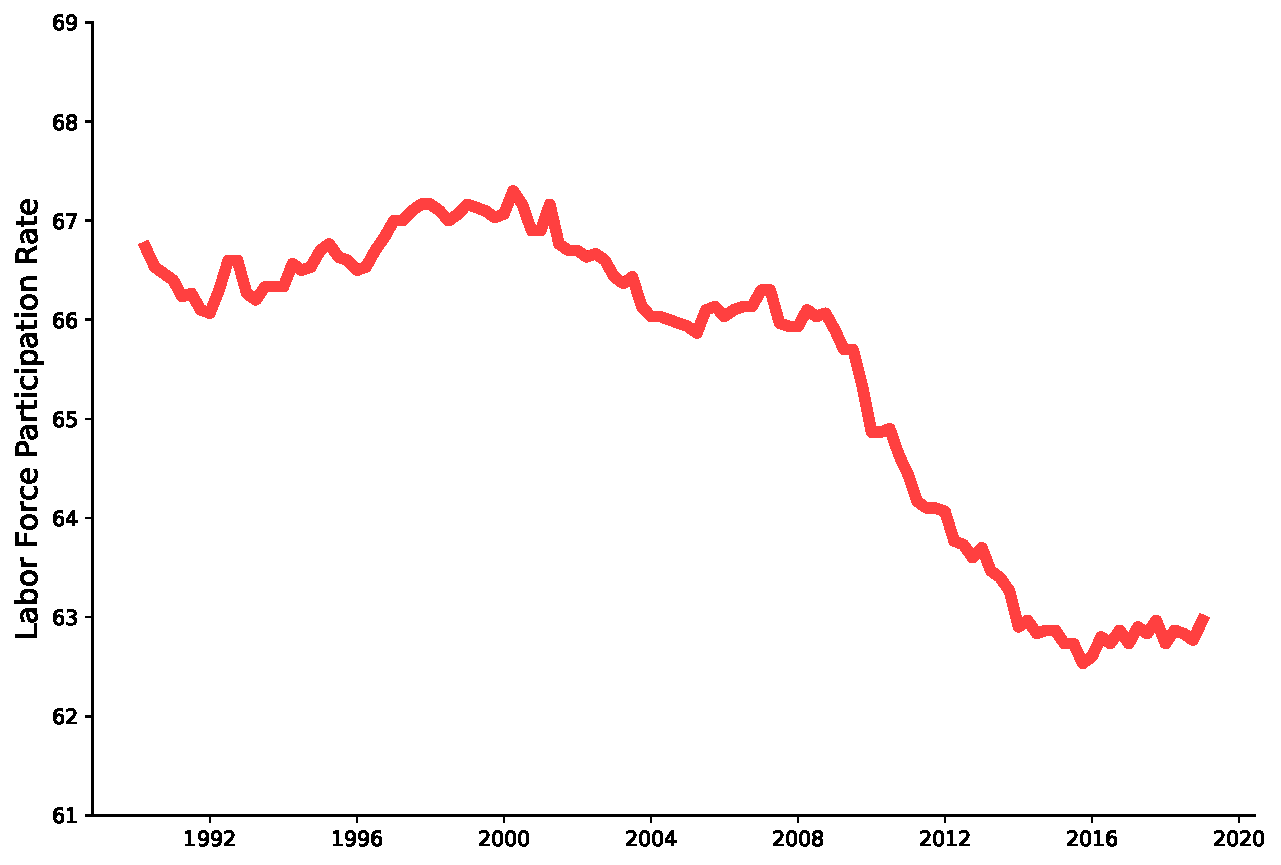
\includegraphics[scale = 0.5]{../figures/participation_rate}
\end{center}
\end{frame}

%%%%%%%%%%%%%%%%%%%%%%%%%%%%%%%%%%%%%%%%%%%%%%%%%%%%%%%%%%%%%%%%%%%%%%%%%%%%%%%%%%%%%%%%%%%%%%%%
%%%%%%%%%%%%%%%%%%%%%%%%%%%%%%%%%%%%%%%%%%%%%%%%%%%%%%%%%%%%%%%%%%%%%%%%%%%%%%%%%%%%%%%%%%%%%%%%

\begin{frame}[t]
\frametitle{Your Friend FRED}
\begin{itemize}
\item Federal Reserve Economic Database (FRED): {\color{blue}\url{http://research.stlouisfed.org/fred2/}}
\begin{itemize}
\medskip
\item Basic tutorials
\medskip
\item Mobile apps
\medskip
\item Excel add-ins for Windows and Mac
\end{itemize}
\medskip
\item Basic graph: Enter code in FRED search box
\medskip
\item Edit graph to change dates, frequency, appearance, units, etc.
\medskip
\item PDF of graph
\medskip
\item Download data into Excel spreadsheet
\end{itemize}
\bigskip
\end{frame}

%%%%%%%%%%%%%%%%%%%%%%%%%%%%%%%%%%%%%%%%%%%%%%%%%%%%%%%%%%%%%%%%%%%%%%%%%%%%%%%%%%%%%%%%%%%%%%%%
%%%%%%%%%%%%%%%%%%%%%%%%%%%%%%%%%%%%%%%%%%%%%%%%%%%%%%%%%%%%%%%%%%%%%%%%%%%%%%%%%%%%%%%%%%%%%%%%

\begin{frame}[t]
\frametitle{FRED Data in Excel}
\begin{itemize}
\item Start at FRED home page
\medskip
\item Graph the first data series that you wish to download
\medskip
\item Click �Edit Graph�
\begin{enumerate}
\medskip
\item Adjust the date range, frequency, units
\medskip
\item Click �Add data series�
\medskip
\item Enter new data code in the search box, repeat step 1 and click �Redraw Graph�
\medskip
\item Repeat steps (1) to (3) until the series are all graphed
\end{enumerate}
\medskip
\item Click �Download Data in Graph�
\medskip
\item Save the Excel file for further analysis of data
\end{itemize}
\bigskip
\end{frame}


%%%%%%%%%%%%%%%%%%%%%%%%%%%%%%%%%%%%%%%%%%%%%%%%%%%%%%%%%%%%%%%%%%%%%%%%%%%%%%%%%%%%%%%%%%%%%%%%%
%%%%%%%%%%%%%%%%%%%%%%%%%%%%%%%%%%%%%%%%%%%%%%%%%%%%%%%%%%%%%%%%%%%%%%%%%%%%%%%%%%%%%%%%%%%%%%%%%
%
%\begin{frame}[t]
%\bigskip
%\bigskip
%\centerline{\huge Bonus Slides}
%
%\end{frame}
%
%
%%%%%%%%%%%%%%%%%%%%%%%%%%%%%%%%%%%%%%%%%%%%%%%%%%%%%%%%%%%%%%%%%%%%%%%%%%%%%%%%%%%%%%%%%%%%%%%%%
%%%%%%%%%%%%%%%%%%%%%%%%%%%%%%%%%%%%%%%%%%%%%%%%%%%%%%%%%%%%%%%%%%%%%%%%%%%%%%%%%%%%%%%%%%%%%%%%%
%
%\begin{frame}[t]
%\frametitle{GDP as Final Sales (Detail)}
%\begin{itemize}
%\item C = final sales to households, ``consumption''
%\begin{itemize}
%\item Durable Goods (lasting at least 3 years)
%\item Non-Durable Goods
%\item Services
%\end{itemize}
%\medskip
%\item I = final sales of capital goods to firms, ``investment''
%\begin{itemize}
%\item Non-Residential Structures
%\item Non-Residential Equipment and Software
%\item Change in Private Inventories
%\end{itemize}
%\medskip
%\item G = purchases of goods and services by government
%\begin{itemize}
%\item Federal Non-Defense
%\item Federal Defense
%\item State and Local
%\end{itemize}
%\medskip
%\item NX = net exports, exports - imports
%\begin{itemize}
%\item Goods
%\item Services
%\item Note: Does note need to be a final sale, i.e. could be and intermediate good.
%\end{itemize}
%\end{itemize}
%\end{frame}
%
%
%%%%%%%%%%%%%%%%%%%%%%%%%%%%%%%%%%%%%%%%%%%%%%%%%%%%%%%%%%%%%%%%%%%%%%%%%%%%%%%%%%%%%%%%%%%%%%%%%
%%%%%%%%%%%%%%%%%%%%%%%%%%%%%%%%%%%%%%%%%%%%%%%%%%%%%%%%%%%%%%%%%%%%%%%%%%%%%%%%%%%%%%%%%%%%%%%%%
%
%\begin{frame}[t]
%\frametitle{Why Care About GDP?}
%\bigskip
%\bigskip
%\begin{itemize}
%\item Bill Easterly, WSJ, March 2007:
%\begin{itemize}
%\medskip
%\item Bill Gates expressed indifference to Africa's stagnant GDP, since ``you can't eat GDP.'' \ldots \\
%    \medskip
%    \textbf{Mr. Gates apparently missed the economics class that listed the components of GDP, such as food.}
%\end{itemize}
%\end{itemize}
%\bigskip
%\end{frame}
%
%%%%%%%%%%%%%%%%%%%%%%%%%%%%%%%%%%%%%%%%%%%%%%%%%%%%%%%%%%%%%%%%%%%%%%%%%%%%%%%%%%%%%%%%%%%%%%%%%
%%%%%%%%%%%%%%%%%%%%%%%%%%%%%%%%%%%%%%%%%%%%%%%%%%%%%%%%%%%%%%%%%%%%%%%%%%%%%%%%%%%%%%%%%%%%%%%%%
%
%
%
%\begin{frame}[t]
%\frametitle{GDP as a Proxy For Well-Being?}
%\bigskip
%\bigskip
%\begin{center}
%\includegraphics[viewport=400 250 0 0, scale=.6]{life}\\ % left, top, bottom, right
%\end{center}
%%\note<1>{\color{granata}\scriptsize GDP, as you have read in the notes, is
%%total value added by residents in a given country. We always think of it as an
%%accurate measure of well-being. Is that so? For sure, well-being is a complex
%%concepts, with many facets. In other words, there are many indicators of well
%%being. How does GDP correlate with them?\\}
%%
%%\note<2>{\color{granata}\scriptsize Life expectancy at birth is nothing but
%%the number of years a new-born is expected to live in a given country. As we
%%can see, it has a strong positive correlation with GDP. There are some
%%outliers, however. The two outliers which have expectancy=50 are South Africa
%%and Equatorial Guinea. \color{blue} For the actual data needed to describe the
%%outliers, refer to the folder in the drawer, or to the web.\\}
%%
%%\note<3>{\color{granata}\scriptsize Issues that should come up here:
%%distribution of income/wealth is very skewed in most developing countries.\\}
%%
%%\note<4>{\color{blue}\scriptsize \color{granata} Talk about Correlation Vs.
%%Causation. Many people think of a causation from GDP to life expectancy. Is it
%%that clear? Any way, the issue to clarify is that: no causation can be
%%inferred from the picture. The figure only outlines a correlation.\\}
%\end{frame}
%
%
%
%%%%%%%%%%%%%%%%%%%%%%%%%%%%%%%%%%%%%%%%%%%%%%%%%%%%%%%%%%%%%%%%%%%%%%%%%%%%%%%%%%%%%%%%%%%%%%%%%
%%%%%%%%%%%%%%%%%%%%%%%%%%%%%%%%%%%%%%%%%%%%%%%%%%%%%%%%%%%%%%%%%%%%%%%%%%%%%%%%%%%%%%%%%%%%%%%%%
%
%\begin{frame}[t]
%\frametitle{GDP as a Proxy For Well-Being?}
%\vspace{-.2in}
%\begin{center}
%\includegraphics[height=2.8in,width=4.25in]{us_france}
%\end{center}
%\end{frame}
%
%%%%%%%%%%%%%%%%%%%%%%%%%%%%%%%%%%%%%%%%%%%%%%%%%%%%%%%%%%%%%%%%%%%%%%%%%%%%%%%%%%%%%%%%%%%%%%%%%
%%%%%%%%%%%%%%%%%%%%%%%%%%%%%%%%%%%%%%%%%%%%%%%%%%%%%%%%%%%%%%%%%%%%%%%%%%%%%%%%%%%%%%%%%%%%%%%%%
%
%
%\begin{frame}[t]
%\frametitle{Flows of Assets}
%\bigskip
%\bigskip
%\begin{itemize}
%\item Allocate flows of assets:
%\begin{eqnarray*}
%Y - C - G &=& I + NX\\
%S &=& I + NX
%\end{eqnarray*}
%\medskip
%\item I $=$ (gross) investment (new plant and equipment)
%\medskip
%\item NX $=$ net purchases of foreign assets
%\medskip
%\item S $=$ (gross) national saving (purchases of assets)
%\end{itemize}
%\end{frame}
%
%%%%%%%%%%%%%%%%%%%%%%%%%%%%%%%%%%%%%%%%%%%%%%%%%%%%%%%%%%%%%%%%%%%%%%%%%%%%%%%%%%%%%%%%%%%%%%%%%
%%%%%%%%%%%%%%%%%%%%%%%%%%%%%%%%%%%%%%%%%%%%%%%%%%%%%%%%%%%%%%%%%%%%%%%%%%%%%%%%%%%%%%%%%%%%%%%%%
%
%\begin{frame}[t]
%\frametitle{Flows of Assets}
%\bigskip
%\bigskip
%\begin{itemize}
%\item Allocate flows of assets:
%\begin{eqnarray*}
%Y - C - G &=& I + NX\\
%S_g + S_p &=& I + NX
%\end{eqnarray*}
%\medskip
%\item I $=$ (gross) investment (new plant and equipment)
%\medskip
%\item NX $=$ net purchases of foreign assets
%\medskip
%\item S $=$ (gross) national saving (purchases of assets) \\ (government + household)
%\begin{itemize}
%\smallskip
%\item $S_g = $ government savings
%\smallskip
%\item $S_p = $ private savings
%\end{itemize}
%\end{itemize}
%\end{frame}
%
%%%%%%%%%%%%%%%%%%%%%%%%%%%%%%%%%%%%%%%%%%%%%%%%%%%%%%%%%%%%%%%%%%%%%%%%%%%%%%%%%%%%%%%%%%%%%%%%%
%%%%%%%%%%%%%%%%%%%%%%%%%%%%%%%%%%%%%%%%%%%%%%%%%%%%%%%%%%%%%%%%%%%%%%%%%%%%%%%%%%%%%%%%%%%%%%%%%
%
%\begin{frame}[t]
%\frametitle{Flows of Assets---U.S. Data}
%\vspace{-.1in}
%\begin{center}
%\includegraphics[height=3.1in,width=4.25in]{savings_netexp_2016}
%\end{center}
%\end{frame}
%
%
%\begin{frame}[t]
%\frametitle{Personal Savings---U.S. Data}
%\vspace{-.1in}
%\begin{center}
%\includegraphics[height=3.1in,width=4.25in]{personal_savings_2016}
%\end{center}
%\end{frame}


\end{document}
